\chapter{Graph Convolutional Networks}

Instead of working with regular grids like image data we can also work with graphs that can be seen as a sort of irregular grids. Graphs differentiate from images and 1d grids that they don't posses a pre-defined order. The nodes of a graph don't have a strictly relative position between one to another. Instead, they are defined by their connections between them. Contrary to images and sequences where all nodes have the same number of neighbors, the number of edges that each node has may be different.

\noindent Graphs can be of different kinds depending on the constrains we impose to them:

\begin{itemize}
    \item Undirected Graphs. Graphs in which edges have no orientation, meaning that they connect two vertices without any indication of direction.
    \item Directed Graphs. Graphs in which each edge is directed from one vertex to another, indicating a one-way relationship between vertices.
    \item Trees. A tree is a connected acyclic graph where any pair of nodes is connected by exactly one path. The top node is known as root, while the peripheral nodes are known as leaves.
\end{itemize}

\begin{figure}[h]
    \centering
    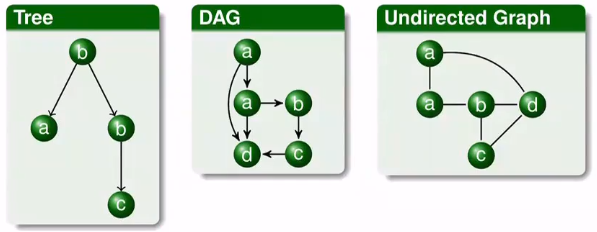
\includegraphics[width=9cm]{Images/types-graphs.png}
    \caption{Different types of graphs}
\end{figure}

\noindent Regression or classification problems with graphs basically consist of given a dataset composed by $N$ pairs $\left ( G_i, y_i \right)$ with $i = (1, ..., N)$ where $N$ is the number of graphs in the dataset, $G_i$ is one graph and $y_i$ is the target/label associated with that graph, the goal is that given an unseen graph $G$ to predict the correct target/label. Each graph $G$ will also have $n_j$ vertices and a vector of attributes $d$ associated to each node.

\newpage

\noindent Graphs are represented with an adjacency matrix $A$. That is a $N \times N$ matrix such that $A_{ij}=1$ if there is an edge between nodes i and j, and $A_{ij} = 0$ otherwise. For an undirected and unweighted network2 the adjacency matrix is binary and symmetric $A_{ij}= A_{ji}$ while this is not the case of a directed graph. In the case of an undirected weighted network the adjacency matrix is not binary $A_{ij}= W_{ij}$ if there is an edge between nodes $i$ and $j$ with weight $w_{ij}$ and $A_{ij}=0$ otherwise. Usually, the adjacency matrix of a weighted network is indicated by $W$, to distinguish it from its binary counterpart $A$ where the network structure is the same but weights are neglected.

\begin{figure}[h]
    \centering
    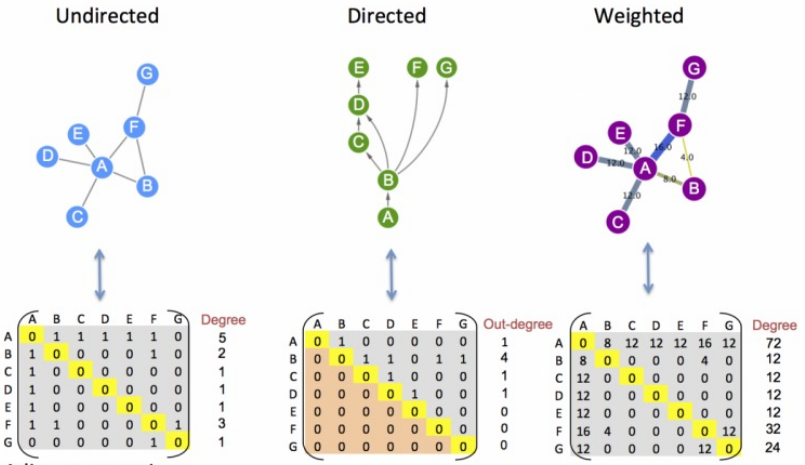
\includegraphics[width=12cm]{Images/adjacency-matrices.png}
    \caption{Different types of adjacency matrices}
\end{figure}







\section{Why is Complicated to Learn with Graphs}

A major problem when working with graphs is that many simple operations that are efficient in other data structures, are computationally very expensive when using graphs. For example just to see if two graphs are isomorphic between each other (if they are the same) or if one graph is a subgraph of another graph is expensive. This is important as when performing learning tasks we use the data of the training set to build our model and then when given a test sample we try to predict the output considering similar data that the model has seen in training. Basically, we exploit the similarities between training and test data. When working with graphs we will not be able to that due to the time complexity of performing these tasks.

\newpage

\section{Micheli Model}

One of the first models proposed to adapt Convolutional Neural Networks to graphs was done by professor Micheli. In this architecture, every node in each layer will model a node in the graph. As a result the network has the same structure as the graph.

\begin{figure}[h]
    \centering
    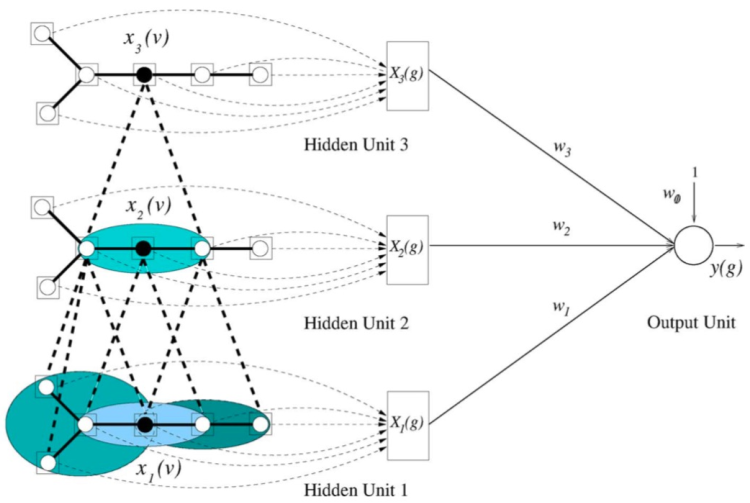
\includegraphics[width=12cm]{Images/nn4g-micheli.png}
    \caption{Architecture of a Neural Network for Graphs proposed by Micheli}
\end{figure}


\noindent A convolution operation is performed in each layer of the network where each convolution takes as input the representation of all previous layers. As in Convolutional Neural Networks the representation computed at a certain layer for a node depends on the same node and its neighbors in the previous layer.

\noindent The representation learned for a node after layer $i$ will be:

$$ h_v^{i} = \sigma \left( \Bar{W}^{i} x_v + W_i \sum_{u \in N(v)} h_{u}^{i-1} \right) $$

\noindent An equivalent matrix formulation:

$$ H^{i} =   \sigma \left(     (\overline{W})^{i} X + W^{i} A H  \right) $$

\noindent Micheli's Graph Neural Network was driven by intuition considering how a Convolutional Neural Network works. Interestingly, we can arrive to a similar formulation following a more formal approach on how to define a convolution operation in a graph.

\newpage
\section{Graph Convolutional Neural Networks}

To extend Convolutional Neural Networks to graphs we will need to exploit the convolution theorem. In the time domain, convolution is an operation that combines two signals to produce a third signal. Mathematically, if we have two signals $f(t)$ and $g(t)$, their convolution $h(t)$ is given by:

$$ h(t) = \int_{-\infty}^{\infty} f(\tau) g(t - \tau) d\tau  $$

which is also represented as $h(t) = f(t)*g(t)$

\noindent In the frequency domain, signals are often represented using their Fourier transforms. The convolution theorem states that the Fourier transform of the convolution of two signals in one domain is equal to the pointwise multiplication of their Fourier transforms. 

$$ F\{f*g\} = F\{f\} \odot F\{g\} $$

\noindent For graphs the Laplacian operator is defined as:

$$  L = I_n - D^{-\frac{1}{2}} A D^{-\frac{1}{2}}$$

\noindent where $A$ is the adjacency matrix and $D$ is a diagonal matrix whose elements represent the degree of each node.

\noindent If the graph is undirected the adjacency matrix is symmetric. Since we can always compute the eigendecomposition in symmetric matrices, we can decompose $L$ as:

$$L = U  \Lambda U^T $$

where $\Lambda$ is a diagonal matrix whose elements are the eigenvalues of the Laplacian matrix and and $U$ is the Fourier basis of the graph.

\noindent Therefore, given a spatial signal $x$, the graph Fourier transform is $\Hat{x} = U^T x$ and the inverse Fourier transform is $x= U \Hat{x}$. Where the graph transform takes you from the graph domain to the spectral domain and the inverse viceversa. By doing this we are able to compute the convolution.

\noindent The convolution between a parametric filter $f_{\theta}$ and a signal $x$ will be defined as:

$$ y = f_{\theta} * x = U \left( \left( U^T f_{\theta} \right) \odot \left( U^T x \right)   \right) $$

where in the frequency domain the convolution is the element-wise multiplication of the Fourier transform of two signals. Since we want the result back to the node domain we apply the inverse Fourier transform $U$.

\noindent Since we don't know how to define the filter in the graph domain, we will work with the filter in the spectral domain $ \hat{f}_{\theta}$ that can be computed as $\hat{f}_{\theta} = U^T f_{\theta}$. Now if we substitute $ f_{\theta}$ in the previous equation we get:

$$ y = f_{\theta} * x = U \left(  \hat{f}_{\theta} \odot \left( U^T x \right)   \right) $$

\noindent We can convert $f_{\theta}$ that is a vector to a diagonal matrix. Doing this we are exploiting the relationship $a \odot b = Ab$ and we will be able to write the convolution operator as:

$$ y = f_{\theta} * x = U \hat{F}_{\theta} U^T x  $$

\newpage
\noindent The filter then can be defined as a polynomial parametric filter using the eigenvalues of the Laplacian matrix:

$$ \hat{F}_{\theta} = \sum_{k=0}^{K} \theta_k \Lambda^K  $$

where $k$ defines the receptive field of the filter.

\noindent Substituting:

$$ y = f_{\theta} * x = U \hat{F}_{\theta} U^T x = \sum_{k=0}^{K} \theta_k U \Lambda^K U^T x = \sum_{k=0}^{K} \theta_k L^k x$$

\noindent By defining the convolution in this way we can compute the convolution directly in the graph domain. Moreover since the Laplacian provides information about random walks in each node we can interpret these filters as encoding random walks in the graph. 

